
\documentclass{article}

\setlength{\parindent}{0pt}
\usepackage{cite}
\usepackage{enumerate}
\usepackage{tikz}
\newcommand\independent{\protect\mathpalette{\protect\independenT}{\perp}}
\def\independenT#1#2{\mathrel{\rlap{$#1#2$}\mkern2mu{#1#2}}}

\begin{document}

\title{Learning Causal Networks in Python}
\author{James Callan}
\date{}

\maketitle

\newpage

\section{Literature Review}

\subsection{Causal Networks}

Causal Networks are graphical models which represent a set of variables, their conditional dependencies, and their causal relationships\cite{verma1990causal} as a Directed Acyclic Graph (DAG) or a Maximal Ancestral Graph (MAG). The nodes of the Graph represent the variables and the edges represent causality, the direction of the edge represents the direction of causality with parent nodes causing child nodes\cite{verma1990causal}. 
\\

In a DAG all edges have a single direction, whereas in a MAG edges may be directed or bidirectional \cite{zhang2008causal}.
\\

\begin{center}
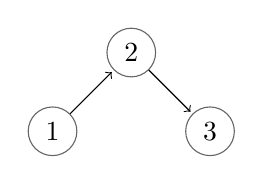
\begin{tikzpicture}[shorten >=1pt,->]
\tikzstyle{vertex}=[circle, draw=black!60, minimum size=12pt]
\node[vertex] (G_1) at (-1,-1) {1};
\node[vertex] (G_2) at (0,0)   {2};
\node[vertex] (G_3) at (1,-1)  {3};
\draw [->] (G_1) -- (G_2);
\draw [->] (G_2) -- (G_3);
\end{tikzpicture}
\end{center}

\begin{center}
Figure 1 A DAG with 3 nodes and 2 edges
\end{center}

\begin{center}
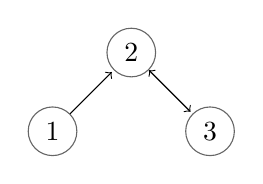
\begin{tikzpicture}[shorten >=1pt,->]
\tikzstyle{vertex}=[circle, draw=black!60, minimum size=12pt]
\node[vertex] (G_1) at (4,-1) {1};
\node[vertex] (G_2) at (5,0)   {2};
\node[vertex] (G_3) at (6,-1)  {3};
\draw [->] (G_1) -- (G_2);
\draw [<->] (G_2) -- (G_3);
\end{tikzpicture}\\
\end{center}

\begin{center}
Figure 2 A MAG with 3 nodes and 2 edges
\end{center}


The learning of causal networks allows relationships between variables to be uncovered and presented in a simple and human readable fashion.
\\

\subsection{Probability and Independence}
In probability theory we can quantify our confidence in a particular event E occurring. This confidence, denoted as P(E) is a real number between 1 and 0 with 1 representing a certainty and 0 representing an impossibility.
\\

In the case of random variables an event would be a variable $X$ taking a particular value $x_1$, where $x_1$ is a member of the set $x = \{x_1, x_2, ..., x_n\}$ of possible values $X$ can take. The probability of this event is denoted as $P(X=x_1)$.
\\

The probability distribution $P(X=x)$ or simply $P(X)$ defines the probabilities for every value which $X$ can take. 
\\

Distributions of more than one variable can be described with joint distributions. For Variables $X$ and $Y$ the distribution $P(X,Y)$  describes the probability of both $X$ and $Y$ taking particular values simultaneously. 
\\

Joint distributions can also describe how the value of one variable can effect the value of an other. $P(X|Y)$ describes the probabilities of $X$ taking particular values ''given'' a value that $Y$ has taken. $P(X|Y) = P(X,Y)/P(Y)$.
\\

If two variables are independent there is no correlation between the values they take. That is for two variables $X$ and $Y$, the distribution $P(X|Y)$ would be the same for all values of $Y$. Therefore $P(X|Y) = P(X)$. If two variables are independent we can determine that there is no causal relationship between them.\\

Two variables $X$ and $Y$ can be considered independent conditioned on a third variable $Z$ if there is no correlation between $X$ and $Y$ for particular values of $Z$.\\


\subsection{D Separation}

A path is any sequence of adjacent edges regardless of their directionality. A collider is node in a path which is both entered and left on edges which are directed toward the node. Unblocked refers to a path that does not traverse a collider\cite{pearl2003causality}.
\\
\begin{center}
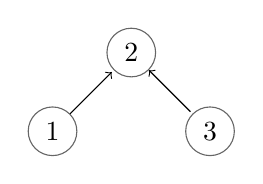
\begin{tikzpicture}[shorten >=1pt,->]
\tikzstyle{vertex}=[circle, draw=black!60, minimum size=12pt]
\node[vertex] (G_1) at (-1,-1) {1};
\node[vertex] (G_2) at (0,0)   {2};
\node[vertex] (G_3) at (1,-1)  {3};
\draw [->] (G_1) -- (G_2);
\draw [<-] (G_2) -- (G_3);
\end{tikzpicture}
\end{center}

\begin{center}
Figure 3 A graph containing a collider
\end{center}

If every path between nodes X and Y traverses a collider, nodes X and Y are unconditionally d-separated or d-separated conditioned on the empty set \cite{pearl2003causality}. Two unconditionally d-separated nodes in a causal network are considered to be independent\cite{pearl2009}.
\\
\begin{center}
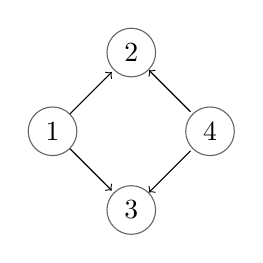
\begin{tikzpicture}[shorten >=1pt,->]
\tikzstyle{vertex}=[circle, draw=black!60, minimum size=12pt]
\node[vertex] (G_1) at (-1,-1) {1};
\node[vertex] (G_2) at (0,0)   {2};
\node[vertex] (G_3) at (0,-2)  {3};
\node[vertex] (G_4) at (1,-1)  {4};
\draw [->] (G_1) -- (G_2);
\draw [<-] (G_2) -- (G_4);
\draw [->] (G_1) -- (G_3);
\draw [<-] (G_3) -- (G_4);
\end{tikzpicture}
\end{center}

\begin{center}
Figure 4
\end{center}

\begin{center}
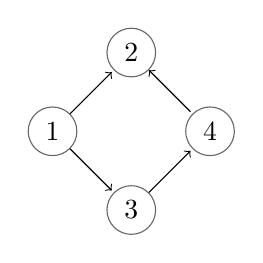
\begin{tikzpicture}[shorten >=1pt,->]
\tikzstyle{vertex}=[circle, draw=black!60, minimum size=12pt]
\node[vertex] (G_1) at (4,-1) {1};
\node[vertex] (G_2) at (5,0)   {2};
\node[vertex] (G_3) at (5,-2)  {3};
\node[vertex] (G_4) at (6,-1)  {4};
\draw [->] (G_1) -- (G_2);
\draw [<-] (G_2) -- (G_4);
\draw [->] (G_1) -- (G_3);
\draw [->] (G_3) -- (G_4);
\end{tikzpicture}
\end{center}

\begin{center}
Figure 5
\end{center}


Two nodes X and Y are d-separated conditioned on set Z if:
\begin{enumerate}
	\item There exists no unblocked path from X to Y that does not traverse any members of Z.\cite{pearl2003causality}
	\item There is no blocked path from X to Y in which all colliders are members of Z or have descendants in Z.\cite{pearl2003causality}
\end{enumerate} 

Causal networks represent conditional independence with d-separation, variables X and Y are conditionally independent on set Z if nodes X and Y are d-separated by nodes in set Z\cite{verma1990causal}.
\\

\subsection{Faithfulness}


By testing for d-separation of variables X and Y given conditioning set Z on a graph we can see if $X \independent Y | Z$ \cite{pearl2009}. However, the reverse is only true if the distribution is faithful to the graph. That is, if a distribution is faithful to a graph then all indpendence relationships are represented on the graph and only these relationships are present \cite{scheines1997introduction}. Assuming faithfulness allows the topology of a graph to be learned by testing pairs of variables for independence given various conditioning sets.
\\

\subsection{Discriminating paths}
For the FCI and RFCI algorithms the notion of discriminating paths is needed. A path $\pi$ = (A, .., X,Y,Z) is discriminating if:
\\

\begin{enumerate}
\item $\pi$ must include at least 3 edges
\item Y is a non-endpoint on $\pi$ and is adjacent to Z on $\pi$.
\item A is not adjacent to Z and every other node is a collider on $\pi$ and a parent of Z. \cite{colombo2012learning} 
\end{enumerate}

\subsection{Algorithms For Learning Causal Networks}
 There have been a number of algorithms developed to learn graphical causal representations from data. Over the course of this project, I plan to implement: The PC algorithm \cite{spirtes1991algorithm}, the Fast Causal Inference (FCI) algorithm \cite{colombo2012learning}, and the Really Fast Causal Inference (RFCI) Algorithm \cite{colombo2012learning}.
\\

Rather than learning an individual DAG the PC algorithm learns a set of DAGs which could represent the causal relationships found in the data. In cases where the direction of an edge is unclear no direction is specified. The output of the algorithm is a partially directed acyclic graph which represents the set DAGs with all possible orientations of undirected edges\cite{spirtes1991algorithm}.
\\

The FCI and RFCI algorithms learn partial ancestral graphs (PAGs) which represent the set of MAGs that fit the data \cite{colombo2012learning}. Unlike in the PC algorithm if the direction of an edge can not be determined it is assumed that there is some set of latent variables influencing the nodes being tested. Each end of an edge can be one of three things in a PAG, an arrow in every MAG ($>$), a tail in every MAG ($-$) or an arrow in at least one MAG and a tail in at least one MAG ($o$), ends of an edge denoted by $*$ can be any of the specified types. This allows for a richer display of information than a partial DAG\cite{colombo2012learning}.
\\
The PAG generated by the FCI algorithm is 
------
than the PAG generated by the RFCI algorithm.
\\

\subsection{Computing a skeleton}
All three algorithms begin by calculating the skeleton of the graph. The skeleton consists of the edges that are present in the partial DAG or PAG however all edges are undirected. When calculating the skeleton the separation set of each pair of variables is recorded \cite{colombo2012learning, spirtes1991algorithm}.
\\

The skeleton is calculated using a series of conditional independence tests. These conditional independence tests are dependent on the type of input data, therefore conditional independence tests can be defined independently of the algorithm.
\\

To begin the skeleton computation the fully connected undirected graph of all variables is constructed and then conditional independence tests are performed to determine which edges to remove.
\\

For the first round of tests, the conditioning set is the empty set Each pair of adjacent variables is tested for independence using some predefined test. For variables X and Y if $X \independent Y$, then the edge X-Y is removed and the empty set is recorded as the separation set (X,Y).
\\

Once all edges have been tested the size of the conditioning set, k, is increased by 1. Now each remaining pair of adjacent variables X and Y are tested for independence given the conditioning set Z. Z is each subset of adj($X$)$\setminus \{Y\}$ of size 1. If any test shows $X \independent Y | Z$ remove the edge X-Y and record Z as the separation set of the pair (X,Y) 
\\

This process is repeated with k being incremented after all edges X-Y have been tested conditioned upon all subsets Z of adj($X$)$\setminus \{Y\}$ of size k. It halts when there are no sets Z of size k for any edge. The edges which have not been removed form the skeleton of the graph which is needed for the PC, FCI and RFCI algorithms along with the recorded separation sets of removed edges \cite{colombo2012learning, spirtes1991algorithm}.
\\

\subsection{The PC Algorithm}
After generating the skeleton and separation sets of pairs of nodes, the pc algorithm attempts to orient the undirected edges of the graph.
\\

It begins by searching for colliders. For each triple of vertices A, B, and C where A and B are adjacent, B and C are adjacent, but A and C are not adjacent orient the edges A-B-C to A$\rightarrow$B$\leftarrow$C if B is not in the separation set of the pair (A,C).
\\

Once colliders are specified other edges can be oriented. This is done by repeating two steps until no more edges can be given a direction:
\\

\begin{enumerate}[i]
  \item If there is is a directed edge from A to B, there is an undirected edge from B to C, and no edge from A to C, orient edge B-C as B$\rightarrow$C.
  \item If there is a directed path from node A to node B and an edge A-B orient the edge as A$\rightarrow$B\cite{spirtes1991algorithm}. 
\end{enumerate}


\subsection{The FCI algorithm}

The FCI algorithm starts in the same way as the PC algorithm using exactly the process of conditional independence tests to estimate a skeleton of the final graph. A list of unshielded triples M must also be found. Unshielded triples are 3 nodes, A, B and C where A and B are adjacent, B and C are adjacent, but A and C are not adjacent. In this skeleton however undirected edges are represented as "o-o". Due to the presence of latent variables this may not be the final skeleton of the graph. It also orients the colliders in a similar way to the pc algorithm, going through all unshielded triples (A,B,C) and orienting the edges $A*-oBo-*C$ as $A*->B<-*C$ if B is not in the seperating set of the pair (A,C).
\\

Next, the final skeleton of the graph is obtained. To do this we must be able to find the possible d-separation set in the graph of a pair of variables X and Y. This set consists of all nodes Z which are colliders on some path $\pi$ between X and Y and on every subpath of $\pi$ (A,B,C) B is a collider or (A,B,C) is a triangle in the graph.
\\

Once the final skeleton has been estimated, repeat the step to orient collider edges on the new skeleton. Finally the edges can be oriented using the rules ($R1-R10$) found in \cite{ZHANG20081873}.\cite{colombo2012learning}
\\


\subsection{RFCI Algorithm}
Like the other two algorithms the RFCI begins by estimating the skeleton of the final graph.
\\

Next the colliders in the graph are found, this is done differently than in the two previous algorithms. We created and empty list L and for each triple (A,B,C) in the list of unshielded triples we check if both:
\\

\begin{enumerate}[i]
	\item $A \independent$ $B$ $|$ $((sepset(A,B) \setminus \{C\})\cup S)$
	\item $B \independent$ $C$ $|$ $((sepset(A,B) \setminus \{C\})\cup S)$\end{enumerate}
where sepset(X,Y) is the separating set of Nodes X and Y and S is the set of selection variables. If both of these tests hold, add to list L. If only the first test holds, find the minimal separating set of A and B and record it as the separating set of A and B. Next, remove the edge A-B, add any newly create unshielded triples to M, and remove any destroyed triples from L and M. If only the second test passes do the same as above but for nodes B and C.
\\

Finally the edges must be oriented. To begin edge orientation apply rules $R1-R3$ found in \cite{ZHANG20081873}. Next triangles (X,Y,Z) must be found with edges $Yo-*Z$, $X<-*Y$, and $X-->Z$. Once a triangle is found the shortest discriminating path from X to Z must be found.
\\

If a path $\pi$ exists take each pair of adjacent variables A and B on $\pi$ and creator a counter $l = 0$. Next find  a subset Y  $\subseteq (sepset(X,Y) \setminus \{A,B\})$ where $|Y| = l$. Then if $A \independent B | Y \cup S$ let sepset(A,B) = Y, delete the edge $A*-*B$ from the graph and update newly formed unshielded triples orientation using the collider orientation described earlier. If the conditional independence test fails increment $l$ and try again, testing with all subsets Y of size $l$, repeat this process until no set Y exists where |Y| = $l$ or the edge $A*-*B$ is removed. 
\\

If no edges are removed from $\pi$ by the above process then either: orient $Yo-*Z$ as $Y-->Z$ if Y is in the sperating set of X and Z or orient $X<-*Yo-*Z$ as $X<->Y<->Z$ if not.
\\

Finally orient as many edges using rules $R5-R10$ from \cite{ZHANG20081873}.
\\

This whole process must be repeated until it no longer alters any orientations.\cite{colombo2012learning}

\bibliography{Report}{}
\bibliographystyle{unsrt}
\end{document}